%%%%%%%%%%%%%%%%%%%%%%%%%%%%%%%%%%%%%%%%%%%%%%%%%%%%%%%%%%%%%%%%%%%%%%%%
% Plantilla TFG/TFM
% Universidad de A Coruña. Facultad de Informática
% Realizado por: Welton Vieira dos Santos
% Modificado: Welton Vieira dos Santos
% Contacto: welton.dossantos@udc.es
%%%%%%%%%%%%%%%%%%%%%%%%%%%%%%%%%%%%%%%%%%%%%%%%%%%%%%%%%%%%%%%%%%%%%%%%


\chapter{Análisis de Viabilidad: Modelado de la Organización.}

\newpage
\section{Formulario OM-1: Contexto Organizacional, problemas y soluciones.}
Identificación de los problemas y oportunidades orientadas al conocimiento de la organización, como se muestra en la Tabla \ref{tab:OM1}.


\begin{table}[H]
\scriptsize
\begin{tabularx}{\textwidth}{|l|X|} \hline
\textbf{Modelo de Organización} & \textbf{Formulario OM-1: Problemas y Posibilidades de Mejora} \\ \hline\hline

\textsc{Problemas y Oportunidades} & El conjunto de medios y/o métodos necesarios para llevar a cabo la organización de una empresa, también conocido como logística, tiene una gran relevancia en la misma. Hemos sido contratados por una empresa de paquetería en España (MRW), con el objetivo de desarrollar un sistema inteligente para mejorar su forma de gestionar los recursos de entrega y recogida de paquetería. Si bien es cierto que esta tarea requiere de un conocimiento adquirido mediante la experiencia, su reiteratividad en muchos aspectos facilita una posible automatización. Actualmente, MRW carece de herramienta o sistema que facilite la tarea de asignación de recursos. \\ \hline
\textsc{Contexto Organizacional} & 
MRW es una importante empresa de paquetería y logística con envíos internacionales de paquetes de diversos tipos, cuya partida hay que planificar, dando continuidad al sistema de automación de la logística de la empresa, que ya cuenta con un sistema de prioridad de entrega según la ruta asignada con el fin de lograr correctamente el cometido: maximizar los recursos que posee la empresa para gestionar las paqueterías que se recibe por parte de la central de MRW con el propósito de entregar/recoger el mayor número de paquetes en el menor tiempo y coste posibles. 

Dicha organización se rige por la obtención del máximo beneficio de la gestión de la paquetería que la franquicia pueda obtener, mientras brinda la mejor calidad del servicio que pueda ofrecer a sus clientes. Además, los valores diferenciales 
con los que identifican son la fiabilidad, calidad, rapidez, innovación, capilaridad, sostenibilidad y cercanía.

La empresa cuenta con 550 franquicias y 58 plataformas logísticas en Andorra, España, Gibraltar y Portugal y realiza una media de 70 millones de envíos anuales. Su modelo organizativo se divide en diversos departamentos con funciones claramente diferenciadas (Facturación, Recepción, Logística, Comercial, RR.HH)\\ \hline
\textsc{Soluciones} & La solución que se propone es desarrollar un sistema que pueda calcular de forma inteligente y óptima los recursos que posee la empresa, es decir, optimizar la gestión de los paquetes que cada vehículo pueda llevar.\\
\hline
\end{tabularx}
  %\label{tab.OM1}
  \caption{\label{tab:OM1}Contexto Organizacional - OM1}
\end{table}
	
 
%%%%%%%%%%%%%%%%%%%%%%%%%%%%%%%%%%%%%%%%%%%%%%%%%%%%%%%%%%%%%%%%%%%%%%%%%%%%%%%
\section{Formulario OM-2: descripción del área de interés de la organización.}

Descripción de los aspectos de la organización que tienen impacto y/o se ven afectados
  por las soluciones basadas en conocimiento elegidas.


\begin{table}[H]
\scriptsize
\begin{tabularx}{\textwidth}{|l|X|} \hline
\textbf{Modelo de Organización} & \textbf{Formulario OM-2: Aspectos Variables} \\ \hline\hline

\textsc{Estructura} & La organización de la empresa MRW se puede ver en la figura (Figura \ref{fig:diagramaEstructura}), donde se puede observar un primer departamento encargado de la dirección del resto de departamentos (Facturación, Recepción, Logística, Comercial y Recursos Humanos). \\ &
\begin{itemize}
  \item Facturación: Departamento encargado de emitir y entregar factura por las actividades realizadas en el desarrollo de la actividad empresarial.
  \item Atención al cliente: Departamento encargado de la atención al cliente, donde esos clientes pueden recoger o entregar paquetes in situ.
  \item Logística: Departamento encargado de todas las actividades relacionadas con la distribución, tanto de los paquetes como de los envíos de la propia paquetería.
  \item Comercial: Departamento encargado de dar a conocer los productos o servicios que comercializa la empresa a través de acciones publicitarias y de promoción, de actualizar los productos en función de las necesidades y cambios en el mercado o de gestionar las relaciones con los clientes.
  \item Recursos Humanos: Departamento encargado de la gestión de los recursos humanos de la organización.
\end{itemize} \\ \hline

\textsc{Procesos} & El proceso de distribución de la paquetería se puede descomponer en X fases principales: \\ &\begin{enumerate}
  \item Recibimiento de los paquetes en la sucursal MRW (entrada).
  \item Generar lista de entregas según ruta asignada.
  \item Determinar los recursos disponibles por la sucursal MRW para entregar según ruta (paquete, personal, transporte, rutas de transporte).
  \item Revisión y validación de la distribución de la paquetería.
\end{enumerate} \\ \hline
\textsc{Personal} &  Los trabajadores encargados de escanear los paquetes para otorgar al sistema información de los mismos y aquellos encargados de repartir en los vehículos (repartidores) pueden o no ser los mismos. Toda la plantilla estaría conformada de trabajadores desde baja cualificación en adelante (sin restricción).

Además, estos estarán liderados por un director.
\\ \hline
\textsc{Recursos} &  Describir los recursos utilizados por los procesos:
\begin{enumerate}
    \item Sistemas de información y otros recursos computacionales:
    \begin{enumerate}
      \item Sistema inteligente.
      \item Base de datos de paquetes.
      \item Base de datos de flota de vehículos.
    \end{enumerate}
    \item Equipamiento y material.
    \begin{enumerate}
      \item Infraestructura informática (escáneres, teléfonos móviles).
      \item Conexión a Internet.
    \end{enumerate}
\end{enumerate}
\\ \hline
\textsc{Conocimiento} &  Experto/s en logística especializado/s en la distribución de paquetería \\ \hline
\textsc{Cultura y Potencial} &  Los colaboradores de la empresa tiene funciones específicas, es decir, hay una persona que se encarga de la atención al cliente, otra persona se encarga de gestionar la logística y los repartidores se encargan de efectuar la entrega/recogida de la paquetería según la ruta asignada por logística. La comunicación, cordialidad y el respeto mutuo es la tónica más importante para el desarrollo de la actividad.\\ \hline
\end{tabularx}
  %\label{tab.OM2}
  \caption{\label{tab:OM2}Descripción del área de interés de la organización - OM2}
\end{table}
\begin{figure}[H]
	\centering
	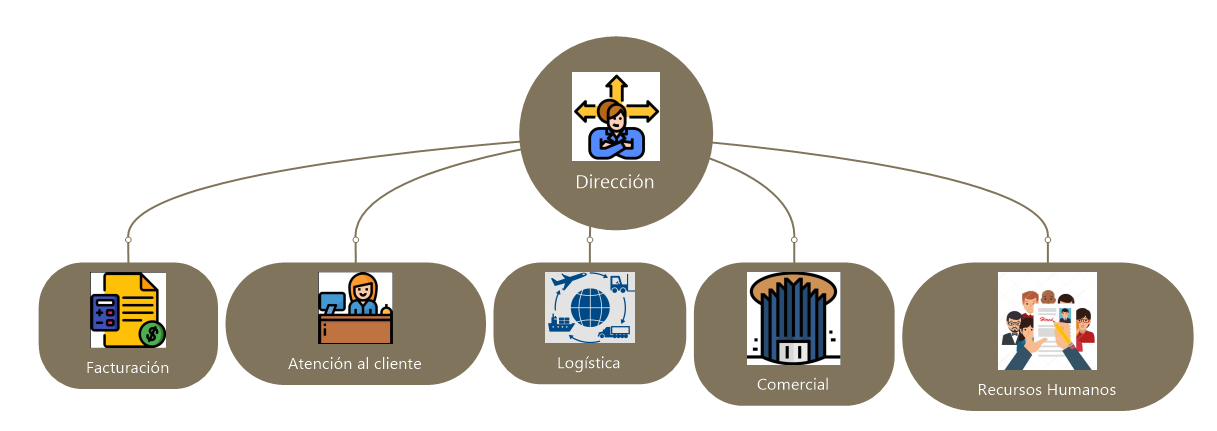
\includegraphics[scale=0.50]{imaxes/Organigrama.png}
	\caption{\label{fig:diagramaEstructura}Diagrama estructura - Formulario OM2}
\end{figure}

\section{Formulario OM-3: Descomposición del Proceso de Negocio.}

Descripción del proceso de interés a partir de las tareas que lo componen.

\begin{table}[H]
  \centering
  \resizebox{15,0cm}{!}{
    \begin{tabular}{|c|c|c|c|c|c|c|}
      \hline
      \multicolumn{3}{|c}{\textbf{Modelo de Organización}} & \multicolumn{4}{|c|}{\textbf{Formulario OM-3: Descomposición de los Procesos}}\\
      \hline \hline
      \textsc{N\textordmasculine} & \textsc{Tarea} & \textsc{Realiza\-da por} & \textsc{¿Dónde?} & \textsc{Recursos de Conocimiento} & \textsc {¿In\-ten\-si\-va en Conocimiento?} & \textsc{Im\-por\-tan\-cia} \\
      \hline

      1 & Recibimiento de los paquetes en la sucursal MRW (entrada) & \multicolumn{1}{|p{3.0cm}|}{\centering Repartidor experimentado} & \multicolumn{1}{|p{3.0cm}|}{\centering En la nave de la sucursal de MRW} & \multicolumn{1}{|p{5.0cm}|}{\centering No } & No & Máxima \\
      \hline
      2 & Generar lista de entregas según ruta asignada & \multicolumn{1}{|p{3.0cm}|}{\centering Repartidor experimentado} & \multicolumn{1}{|p{3.0cm}|}{\centering En la nave de la sucursal de MRW} & \multicolumn{1}{|p{5.0cm}|}{\centering Experiencia en reparto de paquetes según la ruta asignada} & Sí (bajo) & Máxima \\
      \hline
      3 & Determinar los recursos disponibles por la sucursal MRW para entregar según ruta & \multicolumn{1}{|p{3.0cm}|}{\centering Director} & \multicolumn{1}{|p{3.0cm}|}{\centering En la nave de la sucursal de MRW} & \multicolumn{1}{|p{5.0cm}|}{\centering Experiencia en distribución de recursos. Utilizar teoria de programación dinámica} & Sí (elevado) & Máxima \\
      \hline
      4 & Revisión y validación de la distribución de la paquetería & \multicolumn{1}{|p{3.0cm}|}{\centering Director} & \multicolumn{1}{|p{3.0cm}|}{\centering En la nave de la sucursal de MRW} & \multicolumn{1}{|p{5.0cm}|}{\centering Experiencia en reparto de paquetes y distribución de recursos. Utilizar teoria de programación dinámica} & Sí (elevado) & Máxima \\
      \hline      
    \end{tabular}
  }
	\caption{\label{tab:OM3}Descomposición del proceso de negocio - OM3}
\end{table}

\newpage
\section{Formulario OM-4: Activos de Conocimiento}
%%%%%%%%%%%%%%%%%%%%%%%%%%%%%%%%%%%%%%%%%%%%%%%%%%%%%%%%%%%%%%%%%%%%%%%%%%%%%%%

Descripción del componente \textit{conocimiento} del modelo de la organización.

\begin{table}[H]
  \centering
  \resizebox{15,0cm}{!}{
    \begin{tabular}{|c|c|c|c|c|c|c|}
      \hline
      \multicolumn{3}{|c}{\textbf{Modelo de Organización}} & \multicolumn{4}{|c|}{\textbf{Formulario OM-4: Activos de Conocimiento}}\\
      \hline \hline
      \textsc{Recurso de Conocimiento} & \textsc{Pertenece} & \textsc{Usado en} & \textsc{¿Forma Cor\-recta?} & \textsc{¿Lugar Cor\-recto?} & \textsc {¿Tiempo Cor\-recto?} & \textsc{¿Calidad Cor\-recta?} \\
      \hline
      \multicolumn{1}{|p{4.0cm}|}{\centering Experiencia en reparto de paquetes según la ruta asignada} & \multicolumn{1}{|p{3.0cm}|}{\centering Expertos en reparto} & \multicolumn{1}{|p{3.0cm}|}{\centering Tarea 2 de OM-3} & \multicolumn{1}{|p{3.0cm}|}{\centering Si, el conocimiento se puede adquirir con sistema de ubicación por código postal.} & Departamento de logística & - & \multicolumn{1}{|p{3.0cm}|}{\centering Sí, teniendo en cuenta que son aproximaciones.} \\      
      \hline
      \multicolumn{1}{|p{4.0cm}|}{\centering Experiencia en distribución de recursos} & \multicolumn{1}{|p{3.0cm}|}{\centering Expertos en gestionar recursos} & \multicolumn{1}{|p{3.0cm}|}{\centering Tarea 3 de OM-3} & \multicolumn{1}{|p{3.0cm}|}{\centering Si, Utilizar teorias de programación dinámica} & Departamento de logística & - & \multicolumn{1}{|p{3.0cm}|}{\centering Sí, teniendo en cuenta que son aproximaciones.} \\      
      \hline
      \multicolumn{1}{|p{4.0cm}|}{\centering Utilizar teoria de programación dinámica (Fundamentos de algoritmia.\textit{G. Brassard})} & \multicolumn{1}{|p{3.0cm}|}{\centering Director} & \multicolumn{1}{|p{3.0cm}|}{\centering Tarea 4 de OM-3} & \multicolumn{1}{|p{3.0cm}|}{\centering Si, utiliza teorías de programación dinámica de una fuente consultable y con una información distribuible} & Departamento de logística & - & \multicolumn{1}{|p{3.0cm}|}{\centering Sí, es información validada y aceptada.} \\      
      \hline 
    \end{tabular}
  }
	\caption{\label{tab:OM4}Activos de conocimiento - OM4}
\end{table}


\section{Formulario OM-5: Análisis de viabilidad}


Elementos a considerar en el análisis de la viabilidad del proyecto. Nota: para mayor comodidad, en este apartado se puede prescindir del formato ``tabla'' y transformarla en subsecciones (comando subsubsection) manteniendo los mismos epígrafes de la primera columna.

\begin{table}[H]
  \centering
  \resizebox{15.0cm}{!}{
    \begin{tabular}{|l|l|} 
      \hline
      \textbf{Modelo de Organización} & \textbf{Formulario OM-5: Elementos del Documento de Viabilidad}\\ 
      \hline\hline
      \textsc{Viabilidad Empresarial} & \multicolumn{1}{p{15.0cm}|}{Dado a que éste sería el segundo proyecto de nuestra empresa, disponemos de un historial que nos ayude a estimar los beneficios. Hemos aproximado un beneficio económico mínimo del 30\% del coste del capital invertido, así como experiencia y conocimiento en el ámbito empresarial. \newline 
      Al ser los socios aquellos que llevaremos a cabo el desarrollo de este proyecto, estimamos que el coste será de aproximadamente 4.000\euro/mes (teniendo en cuenta alquiler de instalaciones para llevar a cabo el trabajo, dietas, etc) durante un período de 6 meses, resultando en un total de 24.000\euro \ aproximadamente. \newline
      Es un proyecto de alto riesgo para el capital inicial invertido en ese proyecto, puesto que no afectará el funcionamiento de la empresa, ya que la misma ya se encuentra operativa y recibiendo beneficios de un proyecto anterior con las mismas caractarísticas.}\\
      \hline
    \end{tabular}
  }
  \caption{\label{tab:OM5}Formulario OM-5 (Parte 1). Viabilidad Empresarial}
\end{table}

\begin{table}[H]
  \centering
  \resizebox{15.0cm}{!}{
    \begin{tabular}{|l|l|} 
      \hline
      \textbf{Modelo de Organización} & \textbf{Formulario OM-5: Elementos del Documento de Viabilidad}\\ 
      \hline\hline
      \textsc{Viabilidad Técnica} & \multicolumn{1}{p{15.0cm}|}{En la aplicación Especulador Experto, el proceso de especular en los mercados de divisas (Forex) tiene una complejidad elevada debido a que en el sistema tenemos una base de datos de los activos financieros de Forex muy extensa y tendría que estar conectada a tiempo real con las fluctuaciones de los precios de esos activos, lo que provoca que nuestro sistema tenga mucho conocimiento almacenado y varios procesos de razonamiento a realizar. En nuestra aplicación, el tiempo es un recurso crítico, debido a que en un pequeño margen temporal, los valores de los activos involucrados fluctuan y no se puede hacer nada al respecto. \newline
      La calidad de nuestro sistema está basada en los beneficios que podremos conseguir a la larga con nuestra aplicación: si la aplicación produce beneficios, entonces nuestro sistema es válido (siempre ha de comprobarse de manera exhaustiva). Al ser una aplicación desarrollada para pequeños inversores las interfaces tienen que ser lo más simples e intuitivas posibles.} \\
      \hline
    \end{tabular}
  }
  \caption{\label{tab:OM5-2}Formulario OM-5 (Parte 2). Viabilidad Técnica}
\end{table}

\begin{table}[H]
  \centering
  \resizebox{15.0cm}{!}{
    \begin{tabular}{|l|l|} 
      \hline
      \textbf{Modelo de Organización} & \textbf{Formulario OM-5: Elementos del Documento de Viabilidad}\\ 
      \hline\hline
      \textsc{Viabilidad del Proyecto} & \multicolumn{1}{p{15.0cm}|}{El personal tiene el compromiso de llevar a cabo los pasos necesarios para la realización del proyecto, estando así disponibles los recursos necesarios para su realización, ya sea tiempo, presupuesto, equipamiento o el ya mencionado personal, los cuales parten con el conocimiento y capacidades necesarias.\newline
      Las expectativas son realistas, dentro de un marco optimista, para un proyecto novedoso que se incorpora al mercado, el cual busca obtener los mejores resultados posibles. Para lograr todo lo anterior se cuenta con una buena organización y comunicación tanto interna como externa en el proyecto.\newline
      Por último, como ya se ha dicho, al ser un proyecto novedoso, existe la posibilidad de que la aplicación no vaya a tener los mismos éxitos de comercialización que la aplicación anterior desarrollada, pero como se trata de expandir un nuevo mercado y la experiencia de un proyecto similar, creyemos que nos valdrá el esfuerzo en todos los sentidos.} \\
      \hline
    \end{tabular}
  }
  \caption{\label{tab:OM5-3}Formulario OM-5 (Parte 3). Viabilidad del Proyecto}
\end{table}

\begin{table}[H]
  \centering
  \resizebox{15.0cm}{!}{
    \begin{tabular}{|l|l|} 
      \hline
      \textbf{Modelo de Organización} & \textbf{Formulario OM-5: Elementos del Documento de Viabilidad}\\ 
      \hline\hline
      \textsc{Acciones propuestas} & \multicolumn{1}{p{15.0cm}|}{Después del análisis realizado, se ha concluido que se llevará el proyecto adelante, incluyendo éste todas las tareas especificadas en el OM-3 correspondientes al proceso de "Especulación en Mercado de Divisas". \newline
        Los resultados esperados son una mejor gestion del tiempo, para asegurar el mismo beneficio que necesitaba de una persona pendiente del mercado ahorrandonos los nervios y ganando una toma de decisiones mas veloz.\newline
      Las acciones requeridas serian diseñar un motor de inferencia para sustituir al usuario experto para que tome decisiones de forma totalmente autónoma con una mínima entrada de datos que serian el riesgo que estamos dispuestos a asumir y el número máximo de operativas simultaneas a realizar.\newline
      Los riesgos no  sería sólo no lograr el beneficio esperado, ya que el sistema estaría diseñado para no tener mas pérdidas de las asumidas por el usuario.} \\
      \hline
    \end{tabular}
  }
  \caption{\label{tab:OM5-4}Formulario OM-5 (Parte 4). Acciones Propuestas}
\end{table}

\begin{table}[H]
  \centering
  \resizebox{15.0cm}{!}{
    \begin{tabular}{|l|l|} 
      \hline
      \textbf{Modelo de Organización} & \textbf{Formulario OM-5: Elementos del Documento de Viabilidad}\\ 
      \hline\hline
      \textsc{Acciones propuestas} & \multicolumn{1}{p{15.0cm}|}{Después del análisis realizado, se ha concluido que se llevará el proyecto adelante, incluyendo éste todas las tareas especificadas en el OM-3 correspondientes al proceso de "Especulación en Mercado de Divisas". \newline
        Los resultados esperados son una mejor gestion del tiempo, para asegurar el mismo beneficio que necesitaba de una persona pendiente del mercado ahorrandonos los nervios y ganando una toma de decisiones mas veloz.\newline
      Las acciones requeridas serian diseñar un motor de inferencia para sustituir al usuario experto para que tome decisiones de forma totalmente autónoma con una mínima entrada de datos que serian el riesgo que estamos dispuestos a asumir y el número máximo de operativas simultaneas a realizar.\newline
      Los riesgos no  sería sólo no lograr el beneficio esperado, ya que el sistema estaría diseñado para no tener mas pérdidas de las asumidas por el usuario.} \\
      \hline
    \end{tabular}
  }
  \caption{\label{tab:OM5-4}Formulario OM-5 (Parte 4). Acciones Propuestas}
\end{table}
\clearpage